

A partir de la secuencia de puntos rotada, suavizada y resampleada $\ve{r_i}$ calculamos el vector de primeras diferencias normalizado $\ve{d_i}$, donde $\ve{d_i}[j]= \frac{\ve{r_i}[j+1]-\ve{r_i}[j]}{||\ve{r_i}[j+1]-\ve{r_i}[j]||}, \qquad j=1 \dots n-1,  \qquad \ve{d_i}[j] \in \reals^3 $. Este vector será nuestra característica para el gesto, y cada uno de sus elementos representa la dirección relativa entre las posiciones consecutivas del mismo. El vector de primeras diferencias, sin normalizar, nos da una representación equivalente invariante a la traslación. Al normalizar, removemos toda la información de velocidad y escala contenida en la norma de cada vector de dirección, tornando la característica invariante a la velocidad y escala. 

Es importante notar que sin el re-muestreo esta normalización dejaría todavía una cantidad considerable de información de velocidad en la señal, debido a que la cantidad de puntos de muestreo en los segmentos (interpretando la palabra en el sentido de la longitud de arco) donde el usuario realizar el gesto a altas velocidades es más bajo que en aquellos segmentos en donde la mano se mueve más lentamente.

Como una alternativa a los vectores dirección, empleamos también los ángulos de la representación esférica de los vectores dirección, obteniendo una representación $\ve{a_i}$, donde $\ve{a_i}[j]=(\theta,\phi)_j \in \reals^2$.  La coordenada $z$ de la representación esférica se obvia debido a que es siempre $1$ a consecuencia de la normalización previa, y reescalamos los ángulos de manera que  $\theta,\phi \in [-1,1]$.

%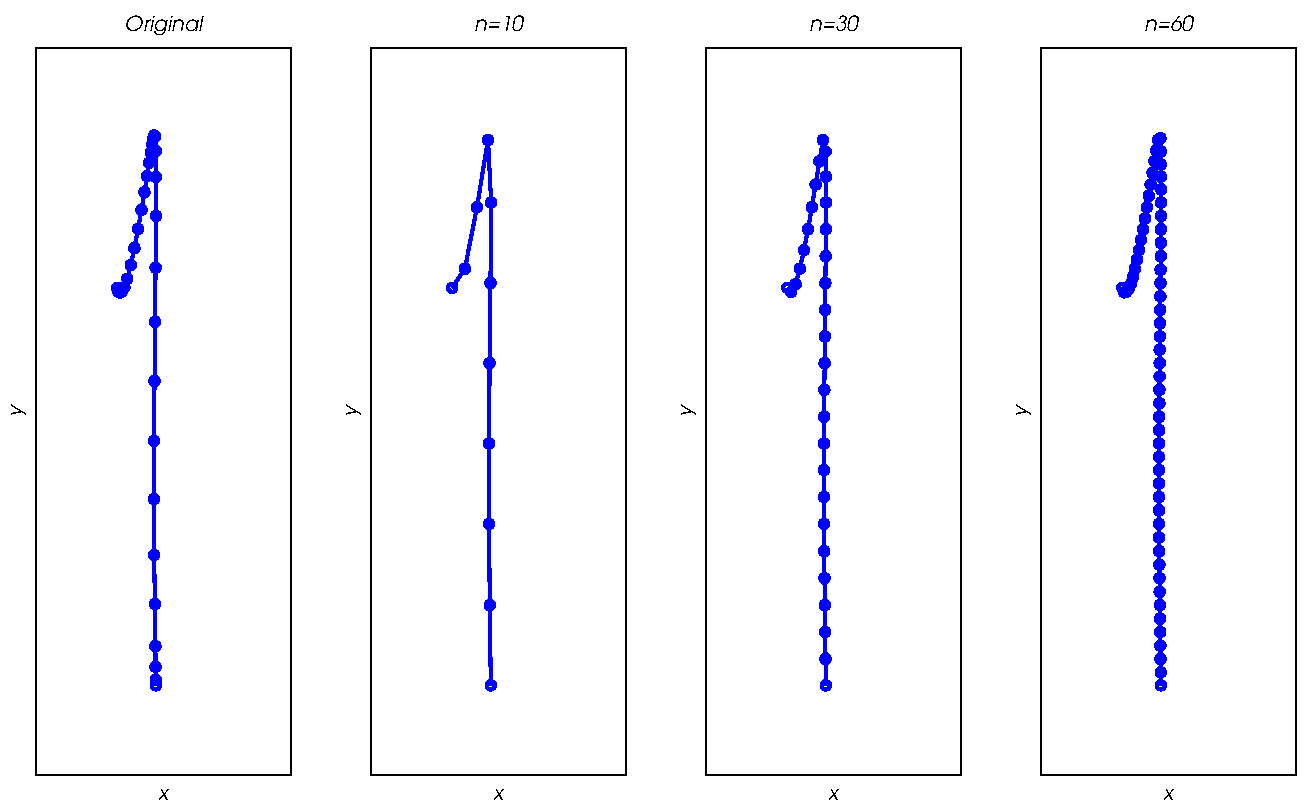
\includegraphics[scale = 0.2]{img/direction}

Dada la naturaleza periódica de la representación con ángulos, en todas las diferencias entre ángulos calculadas para los algoritmos de clasificación utilizamos la función $ d(\alpha,\beta) = min(|\alpha-\beta|, 2- |\alpha-\beta|)$.

Aunque ambas características son isomorfas y tienen las mismas propiedades deseables ( invarianza a la escala, traslación y velocidad \cite{Kindratenko:2003}), producen resultados ligeramente distintos en nuestros experimentos. En las siguientes secciones nos referirmos a las características calculadas a partir de un ejemplar de gesto como $\ve{s}$, donde $\ve{s}[j] \in \reals^d$ puede referirse a cualquiera de las dos características (con $d=2$ para ángulos y $d=3$ para direcciones cartesianas). 


\subsection{Versiones discretas de las propiedades de los gestos}

Previamente definimos un modelo de gestos donde un gesto es una trayectoria continua y hay una relación de equivalencia entre gestos con propiedades deseables. Como los ejemplares son una secuencia de posiciones discretas, necesitamos una versión discreta de dichas propiedades, aplicables a la representación que utilizamos en los algoritmos de clasificación. La principal diferencia entre ambas es la función de correspondencia entre gestos, ya que de todas maneras buscamos una matriz de rotación $\roti$, y constantes de traslación y escala $a$ y $c$. Recordando la definición para el caso continuo:


\equivalencia{ m}{
 & \existsroti, \existsb, \existsa
\\ & c(l) \eequiv a (\roti c'(l))+b
}

Queremos aproximar dicha definición en el caso concreto. Para ello, el resampleo de un gesto nos da una representación de sus posiciones $\ve{r}$ que es uniforme en la longitud total de arco del gesto, y que dado un $n$ lo suficientemente grande, aproxima con error arbitrario a la representación continua.  Entonces, definimos la equivalencia en el caso discreto simplemente como:

\tci{ \rf &\equiv_m \rf' }
{& \existsroti,  \existsb,  \existsa \\ 
& \rf[j] \eequiv  a (\roti \rf'[j])+b, \; \range{j}{1}{n}  }


Como el espacio de búsqueda de dicha transformación es muy grande, buscamos una equivalencia entre características dadas por $ \fdef{\phi}{\ddp}{\mathcal{F}}$, donde $\mathcal{F}$ es el espacio de características, de manera que si $ \phi(\rf) \eequiv \phi(\rf') \tn \rf \equiv_m \rf'$. Es decir, equivalencia en el espacio de las características implica  equivalencia $\equiv_m$.

En nuestro caso, llamaremos  $\phi_d(\xv)=\rf$ a la función característica que dado un ejemplar de gesto realizar la normalización, incluyendo rotación, suavizado y re sampleado, y el cálculo de la primera diferencia con norma 1. 

Debido a la corrección de la rotación, en donde siempre se ubica el cuerpo en cierto sentido, $\phi_d$ es invariante a la rotación. No es invariante a otras rotaciones, ya sean en otras direcciones o de las manos en sí.

Gracias al resampleado y la parametrización por longitud de arco, $\phi_d$ es invariante a la velocidad con la cual fue realizado el gesto, y permite que cada $\rf[j]$ represente siempre la misma parte del gesto, aunque sea de forma aproximada.

El cálculo de la primera diferencia provee invarianza a la traslación, ya que no importan las posiciones absolutas sino las direcciones entre ellas. Llevar dichas diferencias a norma 1 trae invarianza a la escala, ya que así no influye la distancia absoluta entre posiciones contiguas, sino su dirección solamente.

Entonces, nuestra característica $\rf$ es invariante, como deseabamos a la rotación, traslación, velocidad y escala.

Por último, definimos la propiedad de invariancia al punto de comienzo para gestos cerrados discretos, para algún clasificador que pueda implementarla.

En el caso discreto, los gestos cerrados son aquellos para los cuales $x[1] \eequiv x[n]$. Entonces, una característica $\phi$ es invariante a la posición de comienzo si:

\ma{
&\phi(\xv) =\phi( shift(\xv,k)), \quad k=1..n-1  \\
&\text{donde} \\
& \quad shift(\xv,k)=( x_{ (k) \% (n+1)}, x_{ (k+1) \% (n+1)},\dots, x_{ (n+k) \% (n+1)} ) \\
& \quad \text{y \% es el operador \textit{modulo}}
}

La característica $\phi_d$ que desarrollamos en la sección anterior no es invariante al punto de comienzo, debido a que claramente un \textit{shift} de los puntos del gesto causa un \textit{shift} en la característica calculada. El clasificador CNC que describimos en el  capítulo \ref{chap:resultados} \textit{si} provee invarianza al punto de comienzo realizando una transformación posterior a las características obtenidas con $\phi_d$, a costa de perder información sobre la \textit{secuencia} de las direcciones.

En conclusión, hemos definido una característica $\phi_d$ para una secuencia de puntos 3D $\xv$, y establecido que es invariante a la rotación, traslación, velocidad y escala, propiedades de utilidad para el reconocimiento de gestos.